\section{Wykład 2 - wstęp do neurofizjologii $\heartsuit$ $\heartsuit$}

Mózg waga $1250 - 1400\ g$, $100$ mld neuronów, dzienny ubytek $10$ tyś., liczba połączeń $100$ tyś mld,
szerokość synaps ($20-25$ nanometrów - szerokość $\frac{1}{600}$ włosa. Zużycie glukozy $20\%$ większe
niż inne narządy, zużycie tlenu $20\%$, intensywność ukrwienia $750$ ml/min, energii $10$ WAT.

Neuron składa się z dendrytów , jądra komórki (na niej ziarnistości - soma) i aksonu. (na koniec kolaterale końcowe)
Wejścia presynaptyczne (akson) do jądra (neuronu postsynaptycznego).

\paragraph{Rodzaje neuronu}

\begin{enumerate}
 \item jednobiegunowy, dwubiegunowy, gwiaździsty
 \item purkinjego, kłębuszkowy, golgiego
\end{enumerate}

Na końcu aksonu jest synapsa (kolbka synaptyczna). Dotyka ciała komórki odbiorczej. Synapsa składa
się z neurogibryli , mitochondrium, aparatu Golgiego, pęcherzyków synaptycznych i błony pre i post synaptycznej.

Typowy kierunek przemieszczania się sygnału jest od dentrytu do aksonu, ale może następować odwrotny przepływ sygnału.
pojedyncze neurony mogą wysyłać sygnały nawet przy braku
elektrycznej stymulacji w obrębie ciała komórki czy dendrytów.
Procesy pamięciowe komórek zachodzą w aksonach, a potencjał iglicowy jest generowany dalej (bliżej końca aksonu).
Aksony komunikują się ze sobą. 

\paragraph{Schemat funkcjonowania synapsy}

\begin{enumerate}
 \item neurotransmiter
 \item pęcherzyk synaptycznych
 \item enzym rozkładający
 \item receptor presynaptyczny
 \item receptor postsynaptyczny
\end{enumerate}

\paragraph{Neurotransmitery}

\begin{enumerate}
 \item serotonina
 \item acetylocholina
 \item adrenalina
 \item dopamina
\end{enumerate}

\paragraph{Polaryzacja błony komórkowej}

\begin{enumerate}
 \item potencjał spoczynkowy -70mV
 \item potencjał czynnościowy -59mV (od synapsy pobudzającej)
 \item hiperpolaryzacja (od synapsy hamującej) -80mV
\end{enumerate}

Istnieje mechanizm sygnalizacji wstecznej - endokanabinoidy działają wstecz, przemieszczają się
z neuronu postsynaptycznego do presynaptycznego. Hamuje wytwarzanie się neuroprzekaźnika GABA.

\paragraph{Model neuronu McCullocha-Pittsa 1943}

\begin{equation}
  y^{k+1}= 
\begin{cases}
    1,& \text{if } \sum_{i=1}^n w_i x_i^k \ge T \\
    0,              & \text{otherwise}
\end{cases}
\end{equation}

$x_i^k$ - sygnały wejściowe, mówią, czy w chwili $k$ pojawił się sygnał czy nie, $y$ - wyjście neuronu.
$w_i$ może być dodatni (synapsa pobudzająca) i ujemny (hamująca), $T$ jest wartością progową.

\paragraph{Wierny model pojedynczego neuronu}

32000 równań różniczkowych, 19200 parametrów do oszacowania.

\begin{figure}[H]
 \centering
 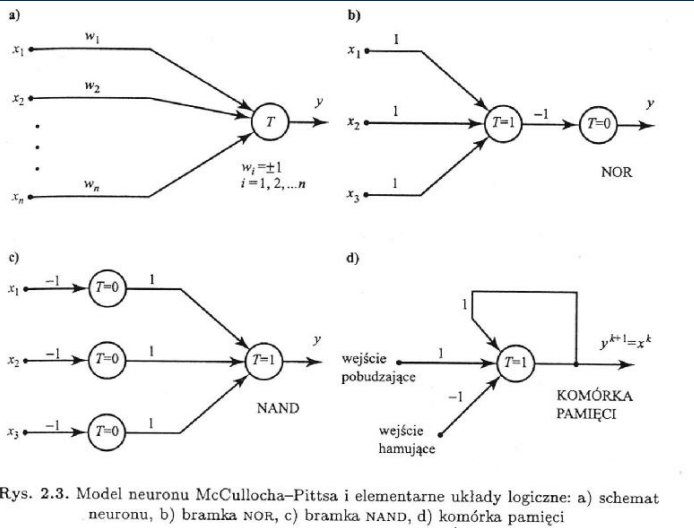
\includegraphics[scale=0.6]{sieci1}
\end{figure}